\documentclass[11pt]{article}
\usepackage{float}
\usepackage{url}
\usepackage{classDM17}
\usepackage{amsmath}
\usepackage{mathtools}

\DeclarePairedDelimiter\ceil{\lceil}{\rceil}
\DeclarePairedDelimiter\floor{\lfloor}{\rfloor}
\newcommand{\BigO}[1]{\mathcal{O}\left( #1 \right)}

\title{Assignment 1: Hash Functions and PAC Algorithms}
\author{Christopher Mertin/\verb~u1010077~\\\url{cmertin@cs.utah.edu}}
\date{\today}

\begin{document}
\maketitle






%%%%%%%%%%%%%%%%%%%%%%%%%%%%%%%%%%%%%%%%%%%%%%%%%%%%
%%%%%%%%%%%%%%%%%%%%%%%%%%%%%%%%%%%%%%%%%%%%%%%%%%%%
%%%%%%%%%%%%%%%%%%%%%%%%%%%%%%%%%%%%%%%%%%%%%%%%%%%%
%\section*{Overview}

%In this assignment you will experiment with random variation over discrete events.  


%It will be very helpful to use the analytical results and the experimental results to help verify the other is correct.  If they do not align, you are probably doing something wrong (this is a very powerful and important thing to do whenever working with real data).  


%\vspace{.1in}

%\emph{As usual, it is highly recommended that you use LaTeX for this assignment.  If you do not, you may lose points if your assignment is difficult to read or hard to follow.  Find a sample form in this directory:
%\url{http://www.cs.utah.edu/~jeffp/teaching/latex/}}

%%%%%%%%%%%%%%%%%%%%%%%%%%%%%%%%%%%%%%%%%%%%%%%%%%%%
%%%%%%%%%%%%%%%%%%%%%%%%%%%%%%%%%%%%%%%%%%%%%%%%%%%%
%%%%%%%%%%%%%%%%%%%%%%%%%%%%%%%%%%%%%%%%%%%%%%%%%%%%
\section{Birthday Paradox (30 points)}

Consider a domain of size $n = 4000$.  

\paragraph{A: (5 points)}
Generate random numbers in the domain $[n]$ until two have the same value.  How many random trials did this take?  
We will use $k$ to represent this value.  

\verb~k = 48~

\paragraph{B: (10 points)}  
Repeat the experiment $m = 300$ times, and record for each time how many random trials this took.  Plot this data as a \emph{cumulative density plot} where the $x$-axis records the number of trials required $k$, and the $y$-axis records the fraction of experiments that succeeded (a collision) after $k$ trials.  The plot should show a curve that starts at a $y$ value of $0$, and increases as $k$ increases, and eventually reaches a $y$ value of $1$.  

\begin{figure}[H]
\centering
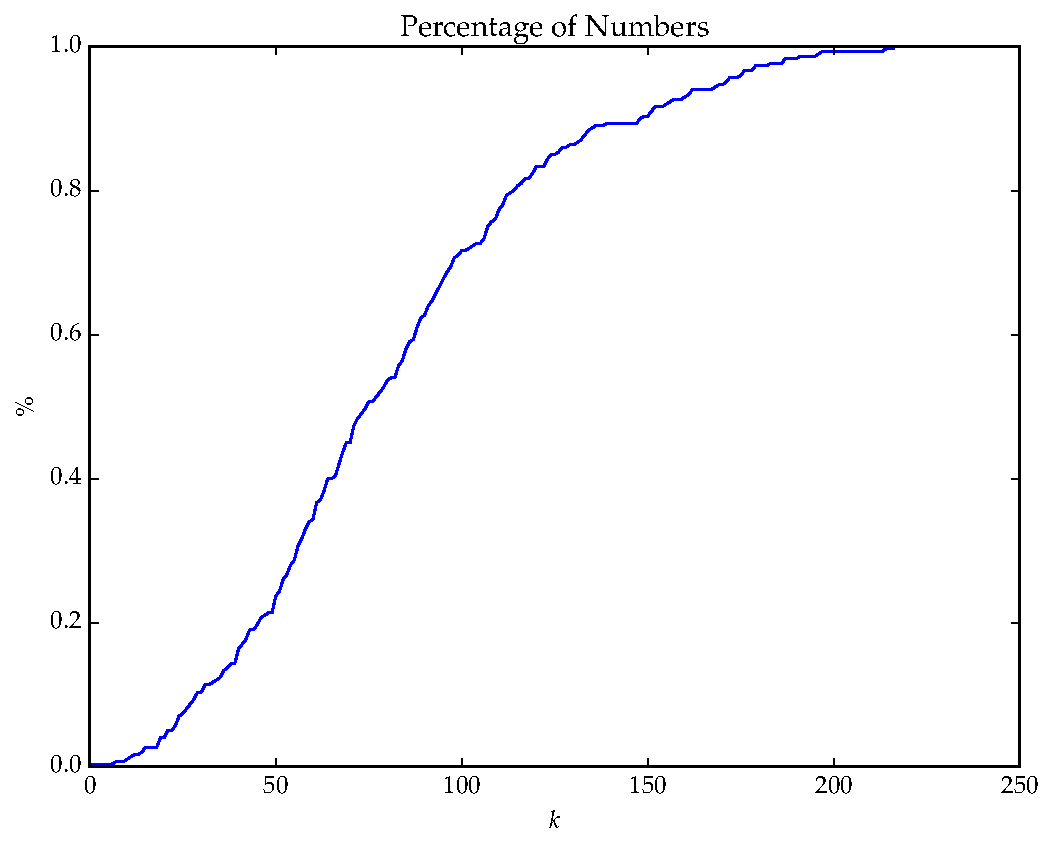
\includegraphics[width=.75\textwidth]{prob1_percentages.pdf}
%\caption{Cumulative density plot with $m = 300$}
\end{figure}

\paragraph{C: (5 points)}  
Empirically estimate the expected number of $k$ random trials in order to have a collision.  That is, add up all values $k$, and divide by $m$.  

\verb~k mean = 78.32~

\paragraph{D: (10 points)}  
Describe how you implemented this experiment and how long it took for $m = 300$ trials.  

Show a plot of the run time as you gradually increase the parameters $n$ and $m$.  
(For at least 3 fixed values of $m$ between 300 and 10,000, plot the time as a function of $n$.)
You should be able to reach values of $n = 1{,}000{,}000$ and $m = 10{,}000$. 

\begin{figure}[H]
\centering
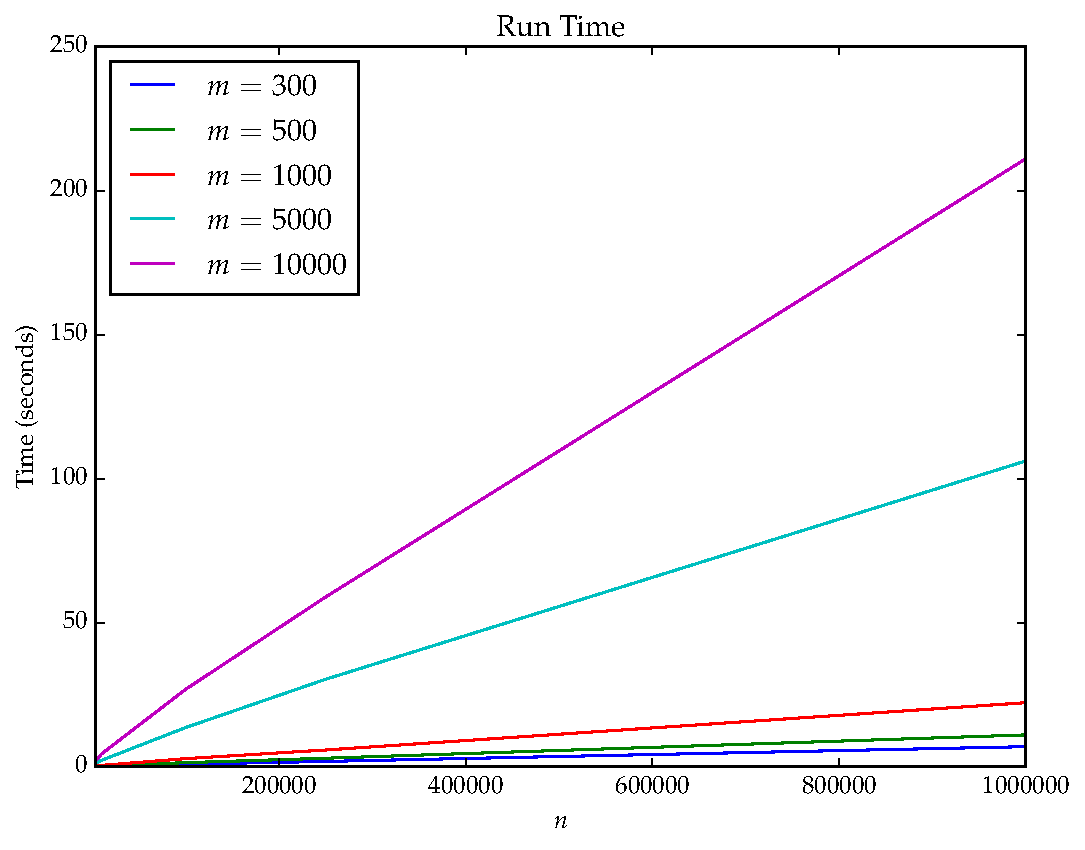
\includegraphics[width=.73\textwidth]{prob1_runtime.pdf}
%\caption{Run time for various values of $m$ and $n$}
\end{figure} 

\begin{figure}[H]
\centering
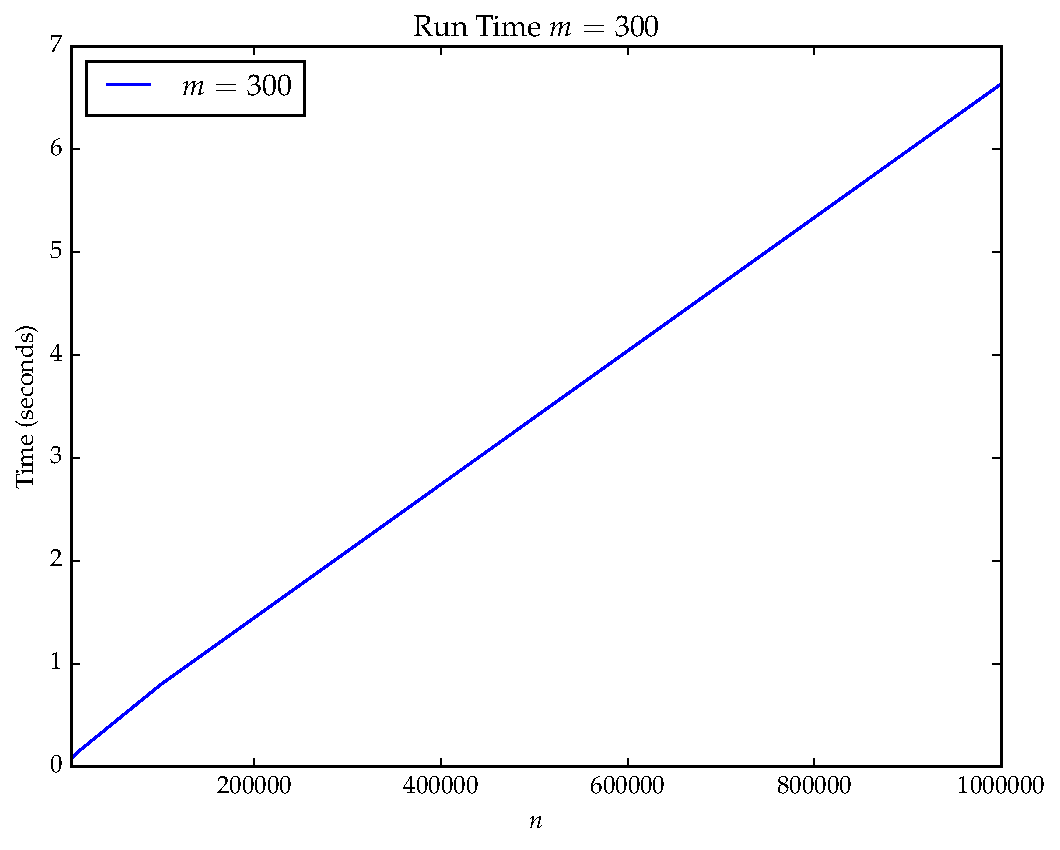
\includegraphics[width=.73\textwidth]{prob1_runtime-m300.pdf}
%\caption{Run time for $m = 300$ over various values of $n$}
\end{figure} 

To implement this code, an empty list was created where each non-matching number would be stored. It would simply append to the list every random number generated in the domain and append it to the list if it was not in the list already.

If it was in the list, the program would end as we would have reached the terminating condition outlined above. The length of the array that stored the numbers was the value of $k$ for that iteration. 

%%%%%%%%%%%%%%%%%%%%%%%%%%%%%%%%%%%%%%%%%%%%%%%%%%%%
%%%%%%%%%%%%%%%%%%%%%%%%%%%%%%%%%%%%%%%%%%%%%%%%%%%%
%%%%%%%%%%%%%%%%%%%%%%%%%%%%%%%%%%%%%%%%%%%%%%%%%%%%
\section{Coupon Collectors (30 points)}

Consider a domain $[n]$ of size $n = 200$.  

\paragraph{A: (5 points)}
Generate random numbers in the domain $[n]$ until every value $i \in [n]$ has had one random number equal to $i$.
How many random trials did this take?  
We will use $k$ to represent this value.  

\verb~k = 1134~

\paragraph{B: (10 points)}
Repeat step $A$ for $m=300$ times, and for each repetition record the value $k$ of how many random trials we required to collect all values $i \in [n]$.  
Make a cumulative density plot as in 1.B.  

\begin{figure}[H]
\centering
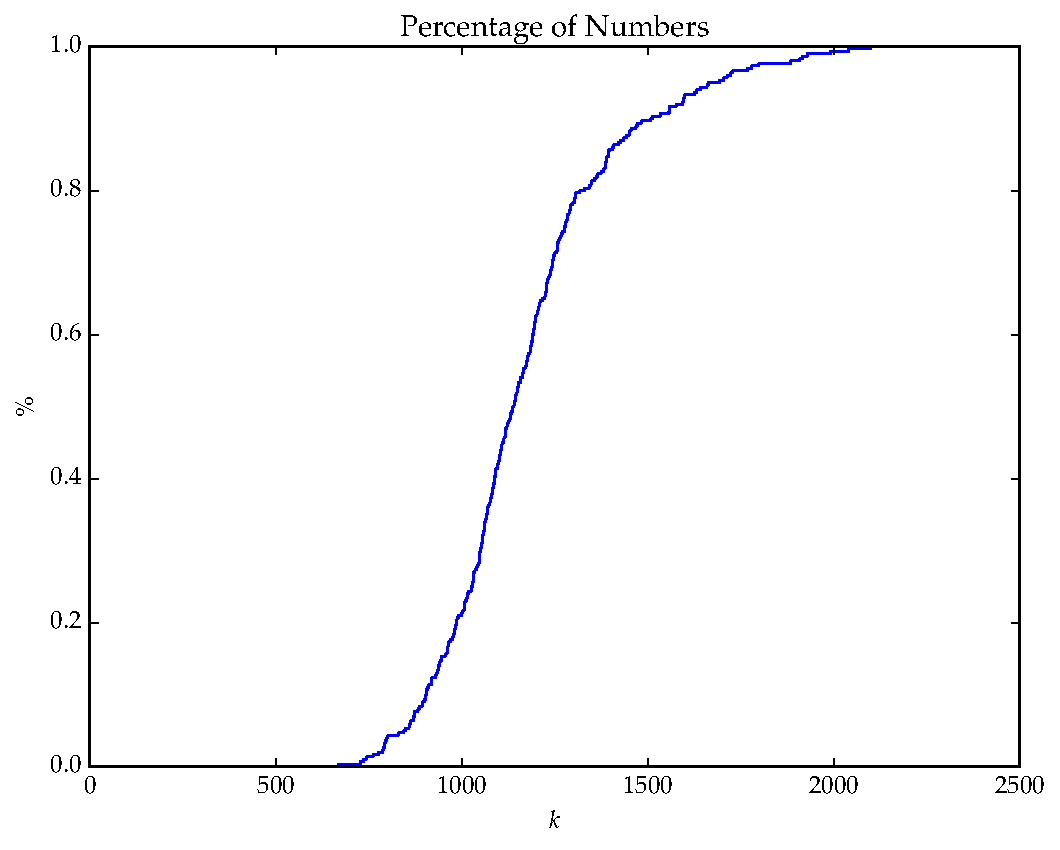
\includegraphics[width=.75\textwidth]{prob2_percentages.pdf}
%\caption{Cumulative density plot with $m = 200$}
\end{figure}

\paragraph{C: (5 points)}
Use the above results to calculate the empirical expected value of $k$.

\verb~k mean = 1184.14~

\paragraph{D: (10 points)} 
Describe how you implemented this experiment and how long it took for $n=200$ and $m=300$ trials.  

Show a plot of the run time as you gradually increase the parameters $n$ and $m$.  
(For at least 3 fixed values of $m$ between 300 and 5,000, plot the time as a function of $n$.)
You should be able to reach $n = 20{,}000$ and $m = 5{,}000$.  

In order to optimize efficienty, the \verb~numpy~ package was used. A \verb~numpy~ array was created at each instantiation of the Coupon Collector problem. The array had dimensions $n + 1$, and each time a random number was created, that index of the array was incremented. After this, the command \\\verb~numpy.count_nonzero(array) == len(array)~ was used as the termiantion sequence for when it was true. This sped up efficiency as the \verb~numpy~ commands are optimized. This would {\em only} be true when every number in the array had a non-zero value.

\begin{figure}
\centering
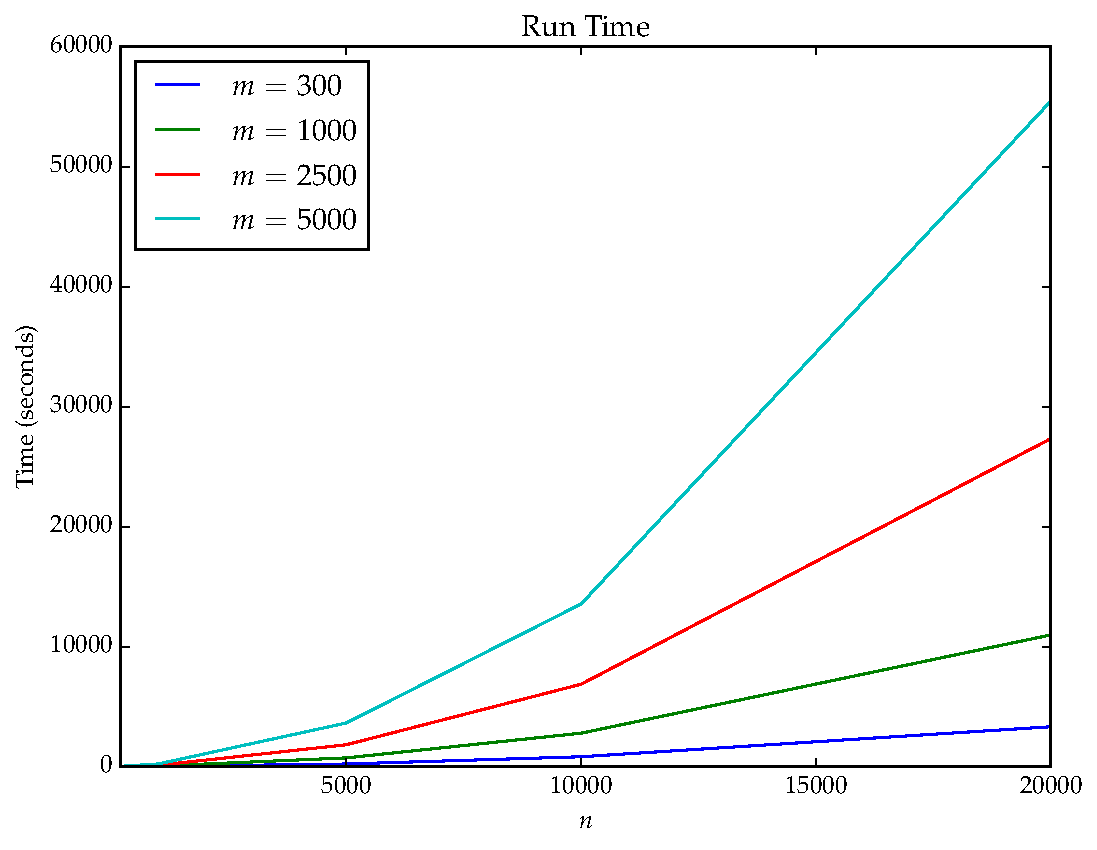
\includegraphics[width=.75\textwidth]{prob2_runtime.pdf}
\end{figure}

\begin{figure}
\centering
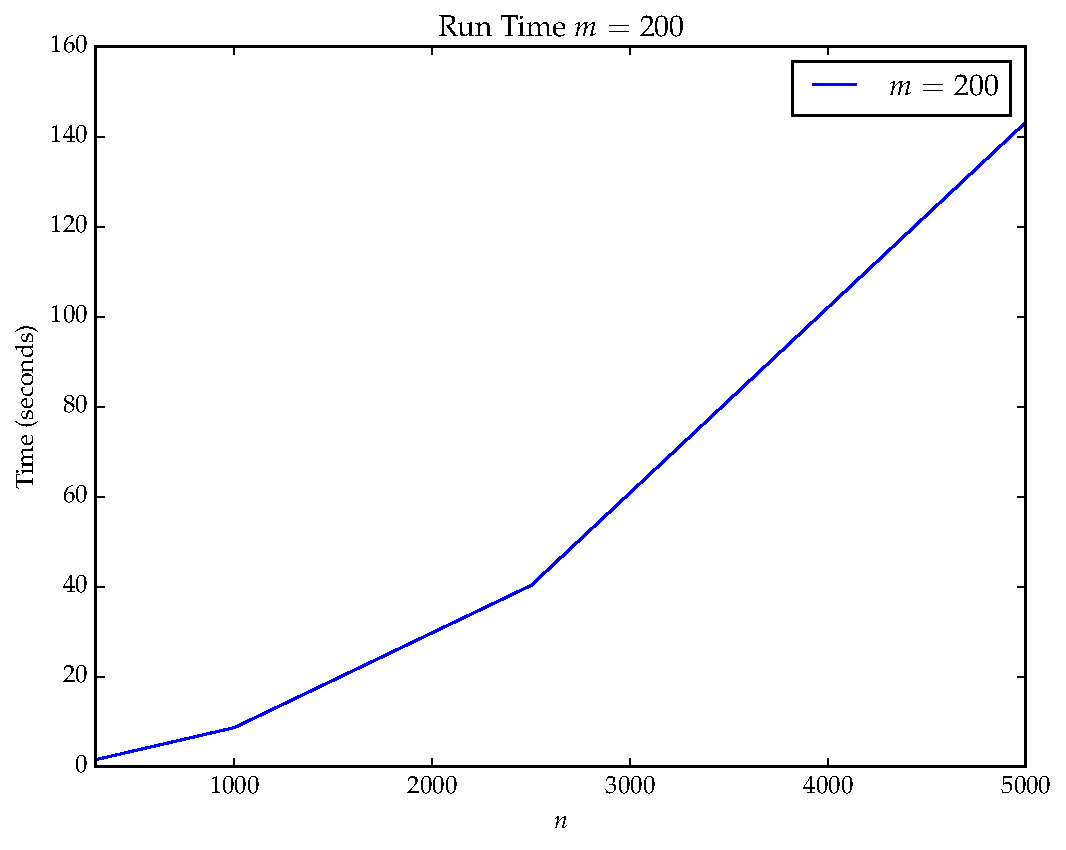
\includegraphics[width=.75\textwidth]{prob2_runtime-m300.pdf}
\end{figure}

%%%%%%%%%%%%%%%%%%%%%%%%%%%%%%%%%%%%%%%%%%%%%%%%%%%%
%%%%%%%%%%%%%%%%%%%%%%%%%%%%%%%%%%%%%%%%%%%%%%%%%%%%
%%%%%%%%%%%%%%%%%%%%%%%%%%%%%%%%%%%%%%%%%%%%%%%%%%%%

\section{Comparing Experiments to Analysis (24 points)}

\paragraph{A: (12 points)}
Calculate analytically (using formulas from the notes in \textbf{L2}) the number of random trials needed so there is a collision with probability at least $0.5$ when the domain size is $n = 4000$.  There are a few formulas stated with varying degree of accuracy, you may use any of these -- the more accurat formula, the more sure you may be that your experimental part is verified, or is not (and you need to fix something).  
\\ \emph{[Show your work, including describing which formula you used.]}

How does this compare to your results from \textsf{Q1.C}?  

The probability of having a collision on the $k^{th}$ iteration in domain $n$ is the product of each individual probability. Therefore, the probability of a collision happening on the $k^{th}$ iteration is

\begin{align*}
p(k) &= 1 - \prod_{i=1}^{k-1}\left(1 - \frac{i}{n}\right)
\intertext{Where, using the Taylor Series Expansion we get}
p(k) &\approx 1 - e^{-k(k-1)/2n}
\end{align*}

From the Taylor Series expansion, we can substitute $n = 4000$ and solve for the required value of $k$ such that the probability is greater than $1/2$. 

\begin{align*}
\frac{1}{2} &\geq 1 - e^{-k(k-1)/2n}\\
\frac{1}{2} &\leq e^{-k(k-1)/2n}\\
\ln\left(\frac{1}{2}\right) &\leq \frac{-n(n-1)}{4000}\\
\intertext{By the Pythagorean Theorem, we get}
0 &= n^{2} + n - 4000\ln\left(\frac{1}{2}\right)\\
n &= 52.16
\end{align*}

Our calculated average was \verb~78.32~, which is relatively close to the actual result. As the number of trials are increased, our accuracy would also increase.

\paragraph{B: (12 points)}
Calculate analytically (using formulas from the notes in \textbf{L2}) the expected number of random trials before all elements are witnessed in a domain of size $n=200$?  Again, there are a few formulas you may use -- the more accurate, the more confidence you might have in your experimental part.  
\\ \emph{[Show your work, including describing which formula you used.]}

How does this compare to your results from \textsf{Q2.C}?

The expected number of random trials needed to generate all values in a domain of size $n$ is defined by

\begin{align*}
T = nH_{n} &= n\left[ \gamma + \ln(n) + \sigma(1/n)\right]\\
       &= n(0.6 + \ln(n))\\
\intertext{For $n = 200$}
T &= 200(0.6 + \ln(200))\\
T &= 1179.66
\end{align*}

The calculated trials in question 2 gave a mean of \verb~1184.14~ which is a really close calulation for only 300 trials. This is most likely due to the fact that there is not going to be a lot of variance in choosing random numbers until every number has a value, as shown in the figure for Question 2 B.

%%%%%%%%%%%%%%%%%%%%%%%%%%%%%%%%%%%%%%%%%%%%%%%%%%%%
%%%%%%%%%%%%%%%%%%%%%%%%%%%%%%%%%%%%%%%%%%%%%%%%%%%%
%%%%%%%%%%%%%%%%%%%%%%%%%%%%%%%%%%%%%%%%%%%%%%%%%%%%
\section{Random Numbers (16 points)}

Consider when the only random function you have is one that choses a bit at random.  In particular \texttt{rand-bit()} returns \texttt{0} or \texttt{1} at uniformly random.  

\paragraph{A: (6 points)}
How can you use this to create a random integer number between $1$ and $n=1024$?  

To create 1024, it requires 10 bits. So you can populate the values of the bits by just calling it $n$ times and assigning the bit value to the current bit.


\paragraph{B: (5 points)}
Describe a Las Vegas randomized algorithm (``Las Vegas'' randomized algorithm means: it may run forever, but you can bound how long you expect it to take, and when it finishes you know it is done and correct) for generating a random number in $[n]$ when $n=1000$.  

You need $\ceil{\log_{2}(n)}$ bits, and consequently that many function calls. For $n = 1000$, we'd need 10 bits. What we would have to do, is randomly assign the bits using the \verb~rand-bit()~ function, and then check to see if the bit string has a value less than $n$. If it does, return that number, if not, rerun it.

\paragraph{C: (5 points)}  
Describe how many \texttt{rand-bit()} calls does the above procedure (extending your algorithm in \textbf{4B}) take as a function of $n$ (say I were to increase the value $n$, how does the number of calls to \texttt{rand-bit()} change)?  

\emph{[Keep in mind that in many settings generating a random bit is much more expensive that a standard CPU operation (like an addition, if statement, or a memory reference), so it is critical to minimize them.  ]}


If we have $n_{1}$ as the first range, and $n_{2}$ as the second range, the difference in the number of calls to \verb~rand-bit()~ would be approximately $\BigO{ \log_{2}(n_{2}) - \log_{2}(n_{1})}$.

\vspace{-.1in}
%%%%%%%%%%%%%%%%%%%%%%%%%%%%%%%%%%%%%%%%%%%%%%%%%%%%
%%%%%%%%%%%%%%%%%%%%%%%%%%%%%%%%%%%%%%%%%%%%%%%%%%%%
%%%%%%%%%%%%%%%%%%%%%%%%%%%%%%%%%%%%%%%%%%%%%%%%%%%%
%\section{BONUS : PAC Bounds (2 points)}

%Consider a domain size $n$ and let $k$ be the number of random trials run, where each trial obtains each value $i \in [n]$ with probability $1/n$.  
%Let $f_i$ denote the number of trials that have value $i$.  
%Note that for each $i \in [n]$ we have $\E[f_i] = k/n$.  
%Let $\mu = \max_{i \in [n]} f_i/k$.  

%Consider some parameter $\delta \in (0,1)$.  
%As a function of parameter $\delta$, how large does $k$ need to be for 
%$\Pr[ |\mu - 1/n| \geq 0.01] \leq \delta$?
%That is, how large does $k$ need to be for \emph{all} counts to be within $1\%$ of the average with probability $\delta$? 
%\emph{(Fine print:  you don't need to calculate this exactly, but describe a bound as a function of $\delta$ for the value $k$ which satisfies PAC property.  Notes here should help: \url{http://www.cs.utah.edu/~jeffp/teaching/cs5140/L2+Chern-Hoeff.pdf})}

%How does this change if we want
%$\Pr[ |\mu - 1/n| \geq 0.001] \leq \delta$ (for $0.1\%$ accuracy)?

%\emph{[Make sure to show your work.]}

\end{document}
